\documentclass[twoside,a4paper]{article}
\usepackage{geometry}
\geometry{margin=1.5cm, vmargin={0pt,1cm}}
\setlength{\topmargin}{-1cm}
\setlength{\paperheight}{29.7cm}
\setlength{\textheight}{24.3cm}

% useful packages.
\usepackage{amsfonts}
\usepackage{amsmath}
\usepackage{amssymb}
\usepackage{amsthm}
\usepackage{enumerate}
\usepackage{graphicx}
\usepackage{multicol}
\usepackage{fancyhdr}
\usepackage{layout}
\usepackage{CJKutf8}
\usepackage{multirow}
\usepackage{rotating,makecell}
\usepackage{verbatim}
\usepackage{indentfirst}  %实现首段首行空两格
\linespread{1.25}%修改行距

\usepackage{graphicx} %插图
\usepackage{float}
\usepackage{diagbox}

% some common command
\newcommand{\dif}{\mathrm{d}}
\newcommand{\avg}[1]{\left\langle #1 \right\rangle}
\newcommand{\difFrac}[2]{\frac{\dif #1}{\dif #2}}
\newcommand{\pdfFrac}[2]{\frac{\partial #1}{\partial #2}}
\newcommand{\OFL}{\mathrm{OFL}}
\newcommand{\UFL}{\mathrm{UFL}}
\newcommand{\fl}{\mathrm{fl}}
\newcommand{\op}{\odot}
\newcommand{\Eabs}{E_{\mathrm{abs}}}
\newcommand{\Erel}{E_{\mathrm{rel}}}

\begin{document}
\begin{CJK*}{UTF8}{gkai}

  \section{问题和相关理论介绍}
  \subsection{问题描述}
  令 $\mathbf x_t\in\mathbb R^m$ 代表时间步 $t$ 处的多变量时间序列的观
  测值。给定一个回溯窗口 $\mathbf X_{t-L:t}=[\mathbf
  x_{t-L},...,\mathbf x_{t-1}]$,目的是预测未来$H$个值 $\hat {\mathbf
    X}_{t:t+H}=[\hat{\mathbf x}_{t},...,\hat{\mathbf
    x}_{t+H-1}]=f(\mathbf X_{t-L:t})$,使得损失最小,即最小化
  $\mathcal L(\hat {\mathbf X}_{t:t+H},\mathbf X_{t:t+H})$。

  \subsection{SCINet模型}
  \begin{figure}[ht]
\centering
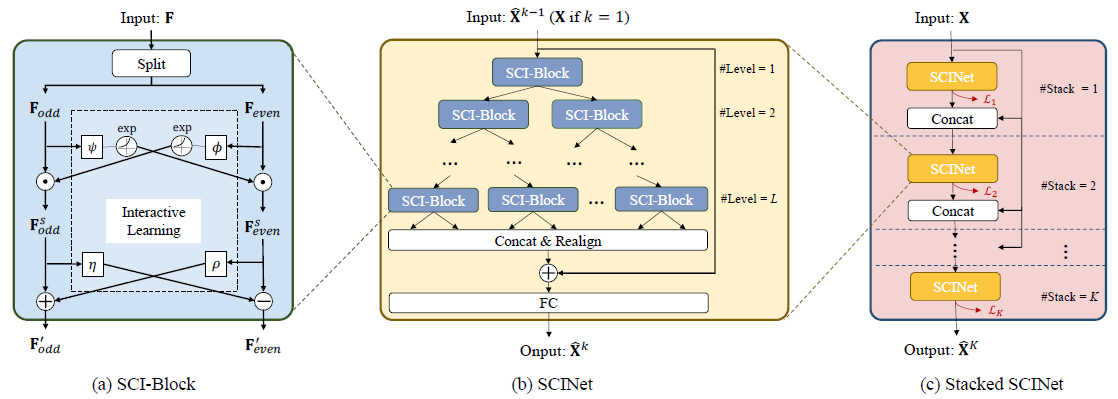
\includegraphics[scale=0.45]{pics/SCINet.png}
\caption{SCINet整体架构}
\end{figure}

SCINet模型是一个分层框架,通过在多个时间分辨率下捕获时间依赖性,增强了
原始时间序列的可预测性。


模型的基本构建块SCI-Block通过奇偶分离将输入数据 $F=[F_1,F_2,F_3,....]$
下采样为两个子序列 $F_{even},F_{odd}$,即
\begin{equation}
  F_{even}=[F_2,F_4,...],\quad F_{odd}=[F_1,F_3,...]
\end{equation}

然后对每个子序列分别使用一组卷积滤波器进行处理,以很好地保留每个子序列的异质性信息。
为了减少下采样过程中信息丢失造成的影响,在使用不同的卷积层从$F_{odd}$
和$F_{even}$中提取特征后,使用一种新的交互学习(Interactive-learning)策
略,允许两个子序列之间进行信息交换。SCINet通过将多个SCI-Block排列成一个二叉树结构来构
建。在所有的下采样-卷积-交互操作之后,我们将所有的低分辨率分量重新排列
到一个新的序列中,使用残差连接后进行预测。

\subsection{时间序列分解}
时间序列分解是指将时间序列分解为几个组分,每个组分表示一类潜在的时间模
式,如季节项(seasonal),趋势周期项(trend-cyclical)。由于预测问题中
未来的不可知性,通常先对过去序列进行分解,再分别预测。

\subsection{DLinear}
  \begin{figure}[ht]
\centering
\includegraphics[scale=0.45]{pics/DLInear.png}
\caption{DLinear整体架构}
\end{figure}

这是第一个挑战Transformer在长期时间序列预测任务中的有效性的工作。
DLinear首先通过移动平均将原始数据输入分解为趋势分量和季节分量。然后,
在每个分量上分别应用两个单线性层,然后将这两个分量相加,得到最终的预测
结果。

\section{我们的模型}
  \begin{figure}[ht]
\centering
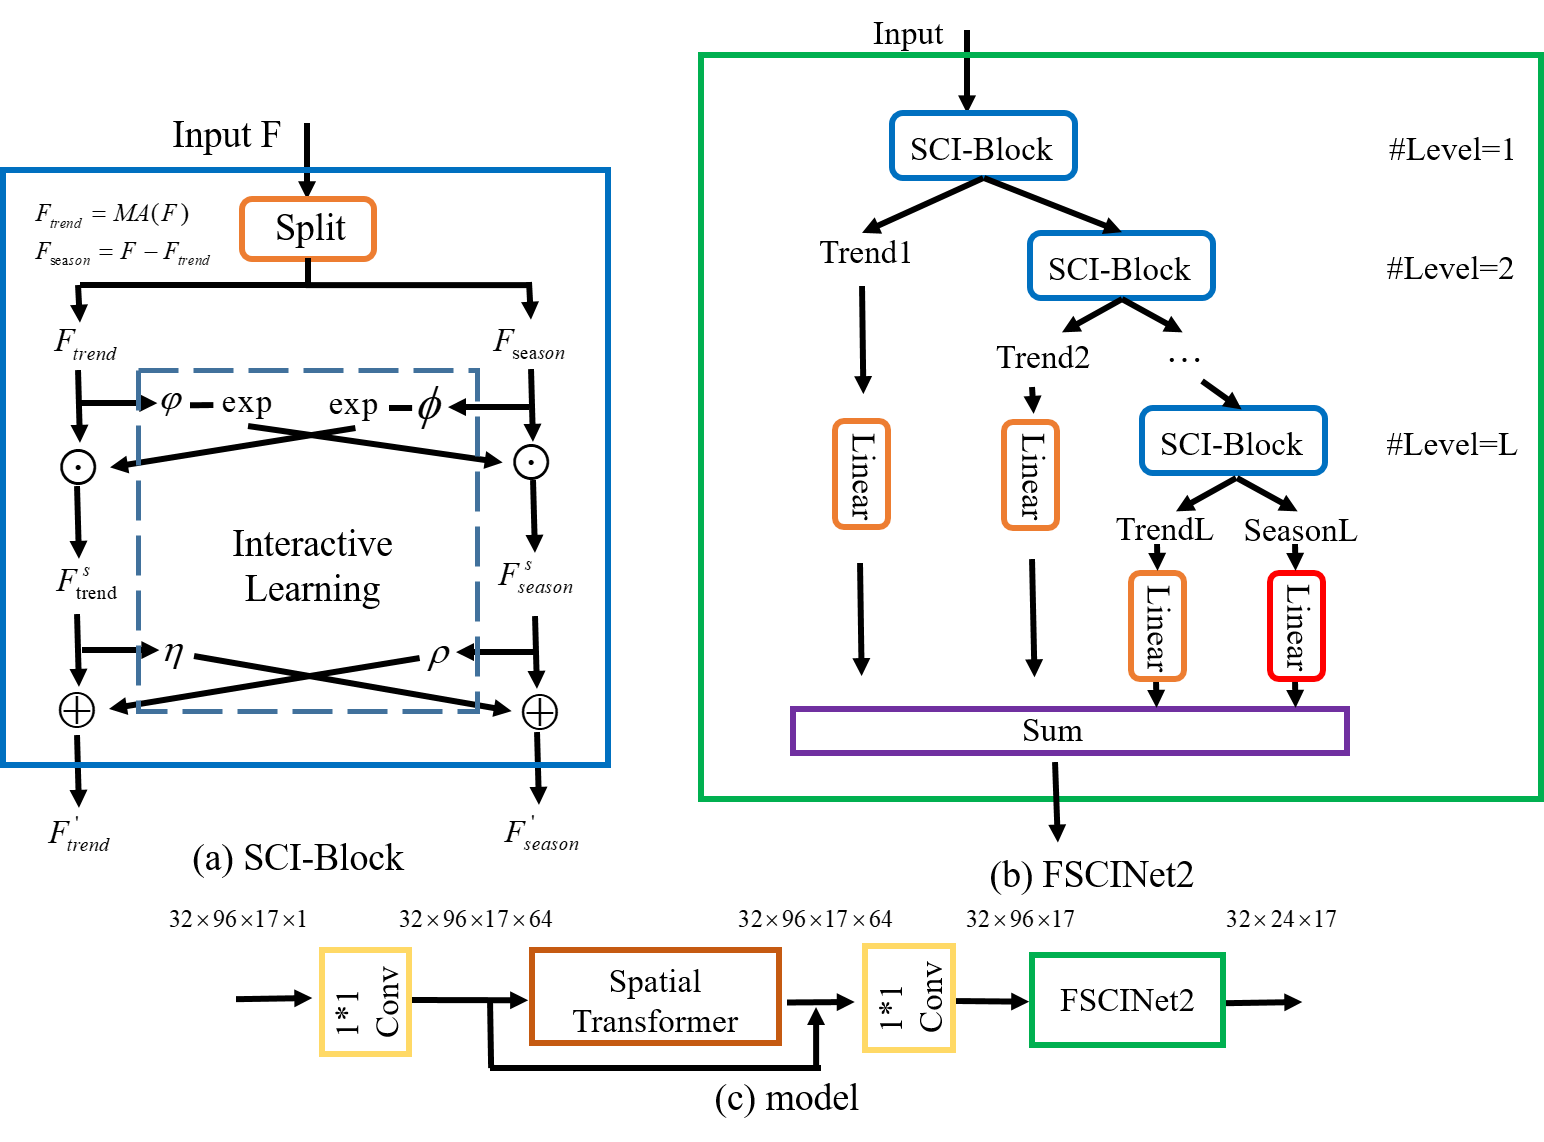
\includegraphics[scale=0.45]{pics/FSCINet2.png}
\caption{模型整体架构}
\label{fig:FSCINet2}
\end{figure}

\subsection{总体架构}
模型的整体架构如图 \ref{fig:FSCINet2} 所示。模型输入为 $X\in \mathbb
R^{L\times N\times C}$,其中 $L$ 为历史序列长度,$N$ 为空间节点数,$C$
为特征数。首先通过一维卷积层得到高维嵌入,接着通过空间Transformer进行空间建模,之后进行残差连接后的结果作为
FSCINet2的输入,FSCINet2的输出也就是模型最后的输出。(因为空间
Transformer直接用的 STTN模型的,故报告里暂未提及)

\subsection{SCI-Block}

SCI-Block是模型的基本模块,它通过Splitting和Interactive-learning的操作,
将输入特征 $F$分解为两个子特征 $F'_{\text{trend}}$ 和
$F'_{\text{season}}$。

我们的模型中的SCI-Block与SCINet模型中的SCI-Block的区别在于Splitting操作。
原始的Splitting操作是将原序列 $F$ 通过奇偶元素分离,下采样为两个低分辨
率子序列 $F_{\text{odd}}$ 和 $F_{\text{even}}$。我们模型的Splitting操
作是通过移动平均操作将 $F$ 分解为趋势分量和季节分量。

\begin{gather}
  F_{\text{trend}}=\text{AvgPool}(\text{Padding}(F))\\
  F_{\text{season}}=F-F_{\text{trend}}
\end{gather}

考虑到两个子序列的异质性信息,我们使用两组不同的卷积层来处理
$F_{\text{trend}}$ 和 $F_{\text{season}}$。


为了进一步补偿每个子序列上的信息,在使用不同的卷积层从
$F_{\text{trend}}$ 和 $F_{\text{season}}$ 中提取特征后,我们依旧采用
SCINet的交互学习(Interactive-learning)策略,以进行两个子序列之间的信息交换。
Interactive-learning通过相互学习仿射变换参数来更新两个子序列,通过耦合
互补部分的信息,可以大大增强学习到的特征的表示能力。


Interactive-learning过程包括两个步骤。

首先,如式(3)所示,用两个不同的一维卷积模块 $\phi$ 和 $\psi$ 分别将
$F_{\text{trend}}$ 和 $F_{\text{season}}$ 投影到隐藏状态,并转换为
$\exp$ 格式,进而进行哈达玛积 $\odot$。这可以看作是在
$F_{\text{trend}}$ 和 $F_{\text{season}}$ 上执行缩放变换,其中使用神经
网络模块相互学习缩放因子。
\begin{gather}
  F_{\text{trend}}^s=F_{\text{trend}}\odot \exp(\phi(F_{\text{season}})),\quad F_{\text{season}}^s=F_{\text{season}}\odot \exp(\psi(F_{\text{trend}})).\\
F_{\text{trend}}'=F_{\text{trend}}^s+\rho(F_{\text{season}}^s),\quad F_{\text{season}}'=F_{\text{season}}^s+\eta(F_{\text{trend}}^s).
\end{gather}
其次,如公式(4)所示,两个缩放后的特征 $F_{\text{trend}}^s$ 和
$F_{\text{season}}^s$ 与另外两个一维卷积模块 $\rho$ 和 $\eta$ 进一步投
影隐藏状态,然后在 $F_{\text{trend}}^s$ 和
$F_{\text{season}}^s$ 上加或减。交互学习模块的最终输出是两个更新后的子
特征 $F_{\text{trend}}'$ 和 $F_{\text{season}}'$ 。 $\phi ,\psi,\rho$
和 $\eta$ 的结构如下图所示,首先会通过repication padding来减少卷积运算
的边界效应,然后采用核大小为 $k$ 的一维卷积将 $C$ 个通道扩展到
$h\ast C$ 个通道,然后进行LeakyRelu和Dropout操作,接着再使用一个一维卷
积层将通道数恢复到 $C$ ,最后使用Tanh激活函数防止负值丢失。

  \begin{figure}[ht]
\centering
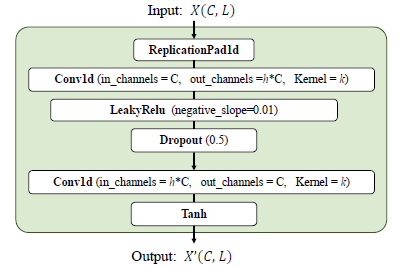
\includegraphics[scale=0.45]{pics/SCINet_p.png}
\caption{The structure of $\phi,\rho,\psi$ and $\eta$.}
\end{figure}

\subsection{FSCINet2}
我们的分解架构类似于小波分解架构,逐层分解出的趋势项经过一个全连接层,
得到这部分的预测结果,季节项继续往下分解直至最后一层,最后的季节项经过
全连接层得到相应的预测分量,最后将这几部分的预测结果加在一起,得到最后的输出。

以 $L=4$ 为例,
\begin{gather}
  F_{\text{trend0}}, F_{\text{season0}} = \text{SCI-Block}(F)\\
F_{\text{trend1}}, F_{\text{season1}} = \text{SCI-Block}(F_{\text{season0}})\\
F_{\text{trend2}}, F_{\text{season2}} = \text{SCI-Block}(F_{\text{season1}})\\
F_{\text{trend3}}, F_{\text{season3}} = \text{SCI-Block}(F_{\text{season2}})
\end{gather}

其中,$F\in\mathbb R^{P\times D}$ 是FSCINet2模型的输入,$P$ 是历史序列
长度,$D$ 是特征数,$Y\in\mathbb R^{Q\times D}$,$Q$ 是预测序列长度。


\subsection{实验结果}
\subsubsection*{时间序列预测}
现如今已经有了许多时间序列预测模型,我们对现有的时间序列预测模型的效果
进行评估。我们已评估的模型有DLinear、NLinear、Transformer、SCINet和我
们模型中的时间模块FSCINet2,评估的数据集包含电力数据集ETTh1、杭州天气
数据集,评估的指标是MSE(均方误差)和MAE(平均绝对误差)。


评估的结果如下所示:
\begin{table}[H]
  \centering
  \caption{单变量ETTh1}
  \begin{tabular}{c c c c c c c c c c c c}
    \hline
    \textbf{Methods} & \multicolumn{2}{c}{FSCINet2}& \multicolumn{2}{c}{SCINet} & \multicolumn{2}{c}{DLinear}
    &\multicolumn{2}{c}{NLinear} &\multicolumn{2}{c}{Transformer}\\
    \hline
    Metrics & MSE & MAE & MSE & MAE & MSE & MAE &MSE & MAE & MSE & MAE \\
    \hline\hline
     24  & 0.0327 & 0.1344 & 0.0375 & 0.1464 & 0.0403 & 0.1528 & 0.0290 & 0.1300 & 0.0651 & 0.2017 \\
     48  & 0.0550 & 0.1744 & 0.0580 & 0.1816 & 0.0537 & 0.1750 & 0.0416 & 0.1560 & 0.1064 & 0.2641 \\
     168 & 0.0925 & 0.2269 & 0.1022 & 0.2424 & 0.0888 & 0.2234 & 0.0740 & 0.2085 & 0.2656 & 0.4413 \\
     336 & 0.1167 & 0.2652 & 0.1241 & 0.2746 & 0.1159 & 0.2653 & 0.0923 & 0.2391 & 0.2757 & 0.4477 \\
     720 & 0.1788 & 0.3486 & 0.1970 & 0.3699 & 0.2082 & 0.3775 & 0.1000 & 0.2492 & 0.2903 & 0.4607 \\
    \hline\hline
  \end{tabular}
  \label{tab:pro_pro}
\end{table}

\begin{table}[H]
  \centering
  \caption{多变量ETTh1}
  \begin{tabular}{c c c c c c c c c c c c}
    \hline
    \textbf{Methods} & \multicolumn{2}{c}{FSCINet2}& \multicolumn{2}{c}{SCINet} & \multicolumn{2}{c}{DLinear}
    &\multicolumn{2}{c}{NLinear} &\multicolumn{2}{c}{Transformer}\\
    \hline
    Metrics & MSE & MAE & MSE & MAE & MSE & MAE &MSE & MAE & MSE & MAE \\
    \hline\hline
     24  & 0.3408 & 0.3737 & 0.3249 & 0.3717 & 0.3620 & 0.3974 & 0.4030 & 0.4196 & 0.5151 & 0.5113 \\
     48  & 0.3800 & 0.4053 & 0.4640 & 0.4008 & 0.3893 & 0.4128 & 0.4314 & 0.4351 & 0.6988 & 0.6355 \\
     168 & 0.4837 & 0.4673 & 0.4640 & 0.4642 & 0.4624 & 0.4568 & 0.5087 & 0.4767 & 0.8903 & 0.7561 \\
     336 & 0.6261 & 0.5553 & 0.5472 & 0.5139 & 0.5175 & 0.4868 & 0.5554 & 0.4996 & 1.1046 & 0.8659 \\
     720 & 0.7800 & 0.6727 & 0.7112 & 0.6278 & 0.5425 & 0.5297 & 0.5556 & 0.5181 & 1.0808 & 0.8306 \\
    \hline\hline
  \end{tabular}
  \label{tab:pro_pro}
\end{table}

\begin{table}[H]
  \centering
  \caption{单变量杭州天气}
  \begin{tabular}{c c c c c c c c c c c c}
    \hline
    \textbf{Methods} & \multicolumn{2}{c}{FSCINet2}& \multicolumn{2}{c}{SCINet} & \multicolumn{2}{c}{DLinear}
    &\multicolumn{2}{c}{NLinear} &\multicolumn{2}{c}{Transformer}\\
    \hline
    Metrics & MSE & MAE & MSE & MAE & MSE & MAE &MSE & MAE & MSE & MAE \\
    \hline\hline
     24  & 0.1248 & 0.2636 & 0.1280 & 0.2673 & 0.1486 & 0.2695 & 0.1354 & 0.2783 & 0.1418 & 0.2847 \\
     48  & 0.1624 & 0.3061 & 0.1661 & 0.3101 & 0.1817 & 0.3301 & 0.1741 & 0.3183 & 0.1692 & 0.3157 \\
     168 & 0.2637 & 0.3957 & 0.2653 & 0.3969 & 0.2705 & 0.4029 & 0.2677 & 0.3933 & 0.2025 & 0.3535 \\
     336 & 0.4089 & 0.5063 & 0.3988 & 0.4986 & 0.3950 & 0.5002 & 0.3980 & 0.4833 & 0.2048 & 0.3551 \\
     720 & 0.7242 & 0.6915 & 0.7142 & 0.6777 & 0.7000 & 0.6846 & 0.8963 & 0.7434 & 0.2001 & 0.3535 \\
    \hline\hline
  \end{tabular}
  \label{tab:pro_pro}
\end{table}

\begin{table}[H]
  \centering
  \caption{多变量杭州天气}
  \begin{tabular}{c c c c c c c c c c c} %c c c c c
    \hline
    \textbf{Methods} & \multicolumn{2}{c}{FSCINet2}& \multicolumn{2}{c}{SCINet} & \multicolumn{2}{c}{DLinear}
    &\multicolumn{2}{c}{NLinear} &\multicolumn{2}{c}{Transformer}\\
    %&\multicolumn{2}{c}{LightTS} &\multicolumn{2}{c}{ETSformer}\\
    \hline
    Metrics & MSE & MAE & MSE & MAE & MSE & MAE & MSE & MAE & MSE & MAE\\
                             % & MSE & MAE & MSE & MAE\\
    \hline\hline
     24  & 0.0958 & 0.2289 & 0.0999 & 0.2333 & 0.1367 & 0.2792 &
                                                                 0.1252 & 0.2637 & 0.1139 & 0.2540\\ %& 0.1019 & 0.2361 & 0.1135 & 0.2532 \\
     48  & 0.1218 & 0.2622 & 0.1324 & 0.2745 & 0.1640 & 0.3072 &
                                                                 0.1584 & 0.2982 & 0.1469 & 0.2902\\ %& 0.1328 & 0.2714 & 0.1452 & 0.2877 \\
     168 & 0.1661 & 0.3123 & 0.1715 & 0.3185 & 0.2458 & 0.3789 &
                                                                 0.2437 & 0.3694 & 0.1743 & 0.3234\\ %& 0.1793 & 0.3211 & 0.2241 & 0.3567 \\
     336 & 0.1707 & 0.3212 & 0.1838 & 0.3319 & 0.3707 & 0.4811 &
                                                                 0.3765 & 0.4664 & 0.1918 & 0.3422\\ %& 0.2313 & 0.3716 & 0.3337 & 0.4388 \\
     720 & 0.2045 & 0.3475 & 0.2140 & 0.3568 & 0.6710 & 0.6692 &
                                                                 0.8771 & 0.7332 & 0.1939 & 0.3453\\ %& 0.4095 & 0.4963 & 0.7444 & 0.6747 \\
    \hline\hline
  \end{tabular}
  \label{tab:pro_pro}
\end{table}

\subsubsection{时空序列预测}

\begin{table}[H]
  \centering
  \caption{STTN}
  \begin{tabular}{c | c c c c | c c c c}
    \hline
    %\hline
    & \multicolumn{4}{c|}{空时(Attn)}& \multicolumn{4}{c}{空时(FSCINet2)}\\
    %\hline
    Metrics & MSE(total) & MAE(total) & MSE(HZ) & MAE(HZ) & MSE(total) & MAE(total) & MSE(HZ) & MAE(HZ) \\
    \hline
     24  & 0.1045 & 0.2429 & 0.1170 & 0.2589 & 0.0940 & 0.2297 & 0.1025 & 0.2430 \\
     48  & 0.1333 & 0.2780 & 0.1491 & 0.2979 & 0.1187 & 0.2601 & 0.1306 & 0.2772 \\
     168 & 0.1777 & 0.3240 & 0.1983 & 0.3450 & 0.1584 & 0.3061 & 0.1770 & 0.3274 \\
     336 & 0.1887 & 0.3386 & 0.1973 & 0.3501 & 0.1738 & 0.3241 & 0.1898 & 0.3458 \\
     720 & 0.2176 & 0.3651 & 0.2286 & 0.3764 & 0.2015 & 0.3501 & 0.2195 & 0.3686 \\
    \hline%\hline
  \end{tabular}
  \label{tab:pro_pro}
\end{table}



\end{CJK*}
\end{document}

%%% Local Variables: 
%%% mode: latex
%%% TeX-master: t
%%% End:




\begin{comment}


\end{comment}

